\documentclass{subfiles}
\begin{document}
\begin{figure}[h!]
    \centering
    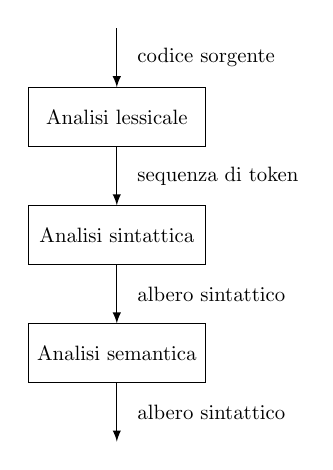
\begin{tikzpicture}[every node/.style={scale=0.75}, scale = 0.75]

        \draw [-latex] (0, 0) -- (0, -1);
        \node (n1) at (0.225, -0.5) [anchor = west] {codice sorgente};

        \draw (-1.5, -1) rectangle (1.5, -2);
        \node (n2) at (0, -1.5) {Analisi lessicale};

        \draw [-latex] (0, -2) -- (0, -3);
        \node (n3) at (0.225, -2.5) [anchor = west] {sequenza di token};

        \draw (-1.5, -3) rectangle (1.5, -4);
        \node (n4) at (0, -3.5) {Analisi sintattica};

        \draw [-latex] (0, -4) -- (0, -5);
        \node (n5) at (0.225, -4.5) [anchor = west] {albero sintattico};

        \draw (-1.5, -5) rectangle (1.5, -6);
        \node (n6) at (0, -5.5) {Analisi semantica};

        \draw [-latex] (0, -6) -- (0, -7);
        \node (n7) at (0.225, -6.5) [anchor = west] {albero sintattico};

    \end{tikzpicture}
    \caption{Struttura di un compilatore.}
    \label{fig:1.1}
\end{figure}
\end{document}